% File: PlanetaryGears.tex
% Author: Adam Leeper
%------------------------------------------------------------------------------
\providecommand{\isolatedBuild}[1]{#1}% Fallback definition to build normally.
\isolatedBuild{
  \documentclass[11pt,letterpaper]{book}
  %\documentclass[11pt,letterpaper]{book}

% aleeper: I think these are needed for Paul's macros?
\usepackage{epsfig}
\usepackage{epstopdf}

%\makeatletter
%\typeout{The import path is \import@path}
%\makeatother

\usepackage{import}

\subimport{./}{packagesMitiguy.sty}
\subimport{./}{macrosMitiguy.tex}
\subimport{./}{PageStylesMitiguy.tex}
\subimport{./}{macrosLeeper.tex}
   % Found via TEXINPUTS environment variable.
  \isolatedBuildHeader{Gears}
                      {A Planetary Gear System}
}
%%%
%%%
%%%
\begin{minipage}{0.5\textwidth}
  The figure to the right shows a \textit{planetary gear system} consisting of
  a central ``sun'' gear A, a ``planet'' gear B whose center is fixed in a
  ``carrier'' frame C, and a ``ring'' gear D.
  The center of the gear box is fixed in a Newtonian frame N.
  %
  \\[0.45pc] We define instantaneous contact points between bodies as follows:
  \\[0.0pc] $A_B$ is the point of A in contact with B;
  \\[0.0pc] $B_A$ is the point of B in contact with A.
  \\[0.0pc] $B_D$ is the point of B in contact with D;
  \\[0.0pc] $D_B$ is the point of D in contact with B.
  \end{minipage}
\hfill
  \begin{minipage}{0.45\textwidth}
  \vspace{-0.1in}
  \flushright
  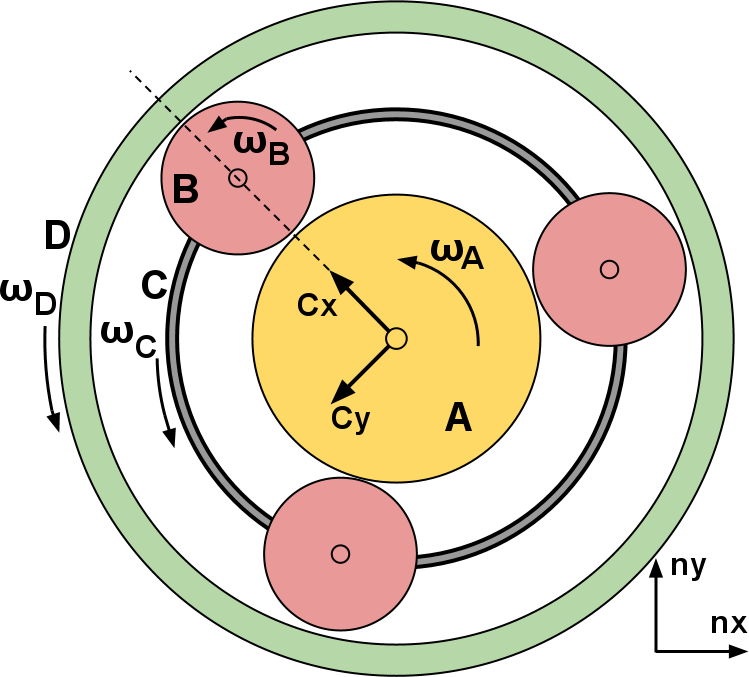
\includegraphics[width=0.9\textwidth]{PlanetaryGear.png}
  \end{minipage}

\begin{minipage}{0.6\textwidth}
   %
   \flushleft
%\begin{center}
{
\small
\begin{tabular}{|l|c|c|}
  \hline Quantity                                                   & Symbol     & Type      % & (Initial) Value(s)
  \\[0.0pc]\hline radius of gear A                                  & $R_A$      & Constant  % & \valueUnits{200}{kg}
  \\[0.0pc]       radius of gear B                                  & $R_B$      & Constant  % & \valueUnits{200}{kg}
  \\[0.0pc]       (inner) radius of gear D                                  & $R_D$      & Constant  % & \valueUnits{200}{kg}
  \\[0.0pc]\hline \uvecz{b} measure of \angvelsDescription{A}{N}    & $\wA$      & Variable  % & \valueUnits{0}{deg}
  \\[0.0pc]       \uvecz{b} measure of \angvelsDescription{B}{N}    & $\wB$      & Variable  % & \valueUnits{0}{deg}
  \\[0.0pc]       \uvecz{b} measure of \angvelsDescription{C}{N}    & $\wC$      & Variable  % & \valueUnits{0}{deg}
  \\[0.0pc]       \uvecz{b} measure of \angvelsDescription{D}{N}    & $\wD$      & Variable  % & \valueUnits{0}{deg}
  \\[0.0pc]\hline
\end{tabular}
}
%\end{center}
   %
   %\\[0.45pc]
   %
\end{minipage}
\hfill
\begin{minipage}{0.4\textwidth}
  You are \boldDarkRed{given} the following:
  \\[0.5pc] $\vel{A_B}{N} = \wA R_A \uvecy{c}$
  \\[0.5pc] $\vel{B_A}{N} = (R_A + R_B) \wC \uvecy{c} - R_B \wB \uvecy{c}$
  \\[0.5pc] $\vel{B_D}{N} = (R_A + R_B) \wC \uvecy{c} + R_B \wB \uvecy{c}$
  \\[0.5pc] $\vel{D_B}{N} = \wD R_D \uvecy{c}$
%  \flushright
%   \vspace{-0.85pc}
\end{minipage}
\\[0.00pc]
%
%
\begin{enumerate}
  \setlength{\itemsep}{0.25pc}
  \item Knowing that gear B \textbf{rolls} on gear A, write a scalar equation relating $\wA$, $\wB$, and $\wC$.
    \\[0.0pc] \textbf{Hint:} First write down the rolling constraint equation.
    %
    \\[0.0pc]\textbf{Result:}\\[-1.35pc]
    %% Adam: Putting half the result here is a pretty huge hint,
    %%       which my students did not receive.
    \begin{displaymath}
       \wA R_A \equals[\;] \hidemath{(R_A + R_B) \wC - R_B \wB}
    \end{displaymath}
    %
    \Solution{\\[0.45pc]}{1.0\linewidth}{
      Since gear \basis{B} rolls on \basis{A}, we can write a constraint
      equation between the velocities of the respective contact points.
      $$\vel{A_B}{N} \equals[\;] \vel{B_A}{N}$$
      $$\wA R_A \uvecy{c} \equals[\;]
        (R_A + R_B) \wC \uvecy{c} - R_B \wB \uvecy{c}$$
      %
      And we then dot with \uvecy{c} to get a scalar relationship:
      \begin{equation}
        \wA R_A \equals[\;] \parens{R_A + R_B} \wC - R_B \wB
      \end{equation}
    }
    %
    \clearpage
  \item Knowing that gear B \textbf{rolls} on gear D, write a scalar equation relating $\wB$, $\wC$, and $\wD$.
    %
    \\[0.0pc]\textbf{Result:}\\[-1.45pc]
    %% Adam: Putting half the result here is a pretty huge hint, which my students did not receive.
    \begin{displaymath}
       \wD R_D \equals[\;] \hidemath{ \parens{R_A + R_B} \wC + R_B \wB}
    \end{displaymath}
    %
    \Solution{\\[0.45pc]}{1.0\linewidth}{
      Since gear \basis{B} rolls on \basis{D}, we write a constraint
      equation between the velocities of the respective contact points.
      $$\vel{B_D}{N} \equals \vel{D_B}{N}$$
      $$\wD R_D \uvecy{c} \equals
        (R_A + R_B) \wC \uvecy{c} + R_B \wB \uvecy{c}$$
      %
      And we then dot with \uvecy{c} to get a scalar relationship:
      \begin{equation}
        R_D \equals \parens{R_A + R_B} \wC + R_B \wB
      \end{equation}
    }
    %
  \item Use your results to part (a) and (b) to find a scalar equation
    relating $\wD$ and $\wC$, \textbf{when the center gear is held fixed}
    in N ($\wA = 0$). Simplify your result by noting that $R_D = R_A + 2 R_B$.
    %
    \\[0.0pc]\textbf{Result:}\\[-1.45pc]
    %
    \begin{displaymath}
    	 \wD = 2 * \parens{\hidemath[1.0cm]{1 \plus[\;] \frac{R_A}{R_D}}} * \wC
    \end{displaymath}
    %
    \Solution{\\[0.45pc]}{1.0\linewidth}{
      Adding equation (1) and (2) yields:
      $$\wD R_D + \wA R_A \equals 2 (R_A + R_B) ~\wC + \wB R_B - \wB R_B$$
      \begin{displaymath}
        \wD R_D \equals 2 (R_A + R_B) ~\wC - \wA R_A
      \end{displaymath}
      Setting $\wA = 0$ and then solving for $\wD$ yields:
      $$\wD \equals \frac{ 2 R_A + 2 R_B}{R_D} \wC$$
      Substituting $R_D = R_A + 2 R_B$, and writing the numerator to make
      it obvious how to split the fraction, yields:
      $$\equals \frac{ R_A + R_A + 2 R_B}{R_A + 2 R_B} \wC$$
      \begin{displaymath}
        \wD \equals \parens{1 + \frac{ R_A }{ R_D }} \wC
      \end{displaymath}
    }
    %
  \item \TrueFalse{0} (circle one).
    It is possible to get the result in (c) if you were instead given only
    $\vel{A_B}{C}$, $\vel{B_A}{C}$, $\vel{B_D}{B}$, $\vel{D_B}{B}$.
    \\[0.0pc] Explain \textbf{briefly}:
    \\[0.0pc]\textbf{Result:}
    %
    \Solution{\\[0.45pc]}{1.0\linewidth}{
%      \\[1.0pc]
      It is valid to write a rolling constraint as long as the
      velocities of the two contact points in the constraint equation are
      in the same frame.
      Hence $\vel{A_B}{C} \equals[\;] \vel{B_A}{C}$ is a valid constraint,
      and $\vel{B_D}{B} \equals[\;] \vel{D_B}{B}$ is also valid.
      While the individual scalar equations resulting from these constraints
      might look slightly different, combining them would still lead to the
      same result as in (c).
    }
\end{enumerate}
%
\isolatedBuildFooter

